%!TEX root = paper.tex

The problem we will analyze in this paper is that of a billiard ball bouncing around inside a square billiard table in the absence of any external forces (e.g. gravity) and/or any dissipative forces (e.g. friction). Before delving into the analysis, we must first clarify the problem statement.

\subsection{Setup}

The ball and table will be idealized in the following manner: we will represent the ball as a point moving around in $\R^2$ and the board as the unit square $[0,1]^2$. The ball will start with an initial position $\bvec{x}_0 \in [0,1]^2$ and initial velocity $\bvec{u}_0$. Because there are no external forces and/or dissipative forces, the speed of the ball is constant and irrelevant to the problem.

Any time the position of the ball (point) coincides with the edge of the table (unit square), we will say that the ball collides with that edge of the table. During this collision, the ball is reflected off the edge of the table in such a manner that the outgoing direction vector is a reflection of the incoming direction vector across the line perpendicular to the edge of the table at the point of collision. In more technical terms, the angle of incidence is equal to the angle of reflection in all ball-table collisions. Collisions at corners of the table are undefined and so we will ignore any such trajectories that intersect corners of the table. Figure \ref{fig:collision-angle} shows the general mechanics of a collision.

\begin{figure}[H]
  \begin{center}
    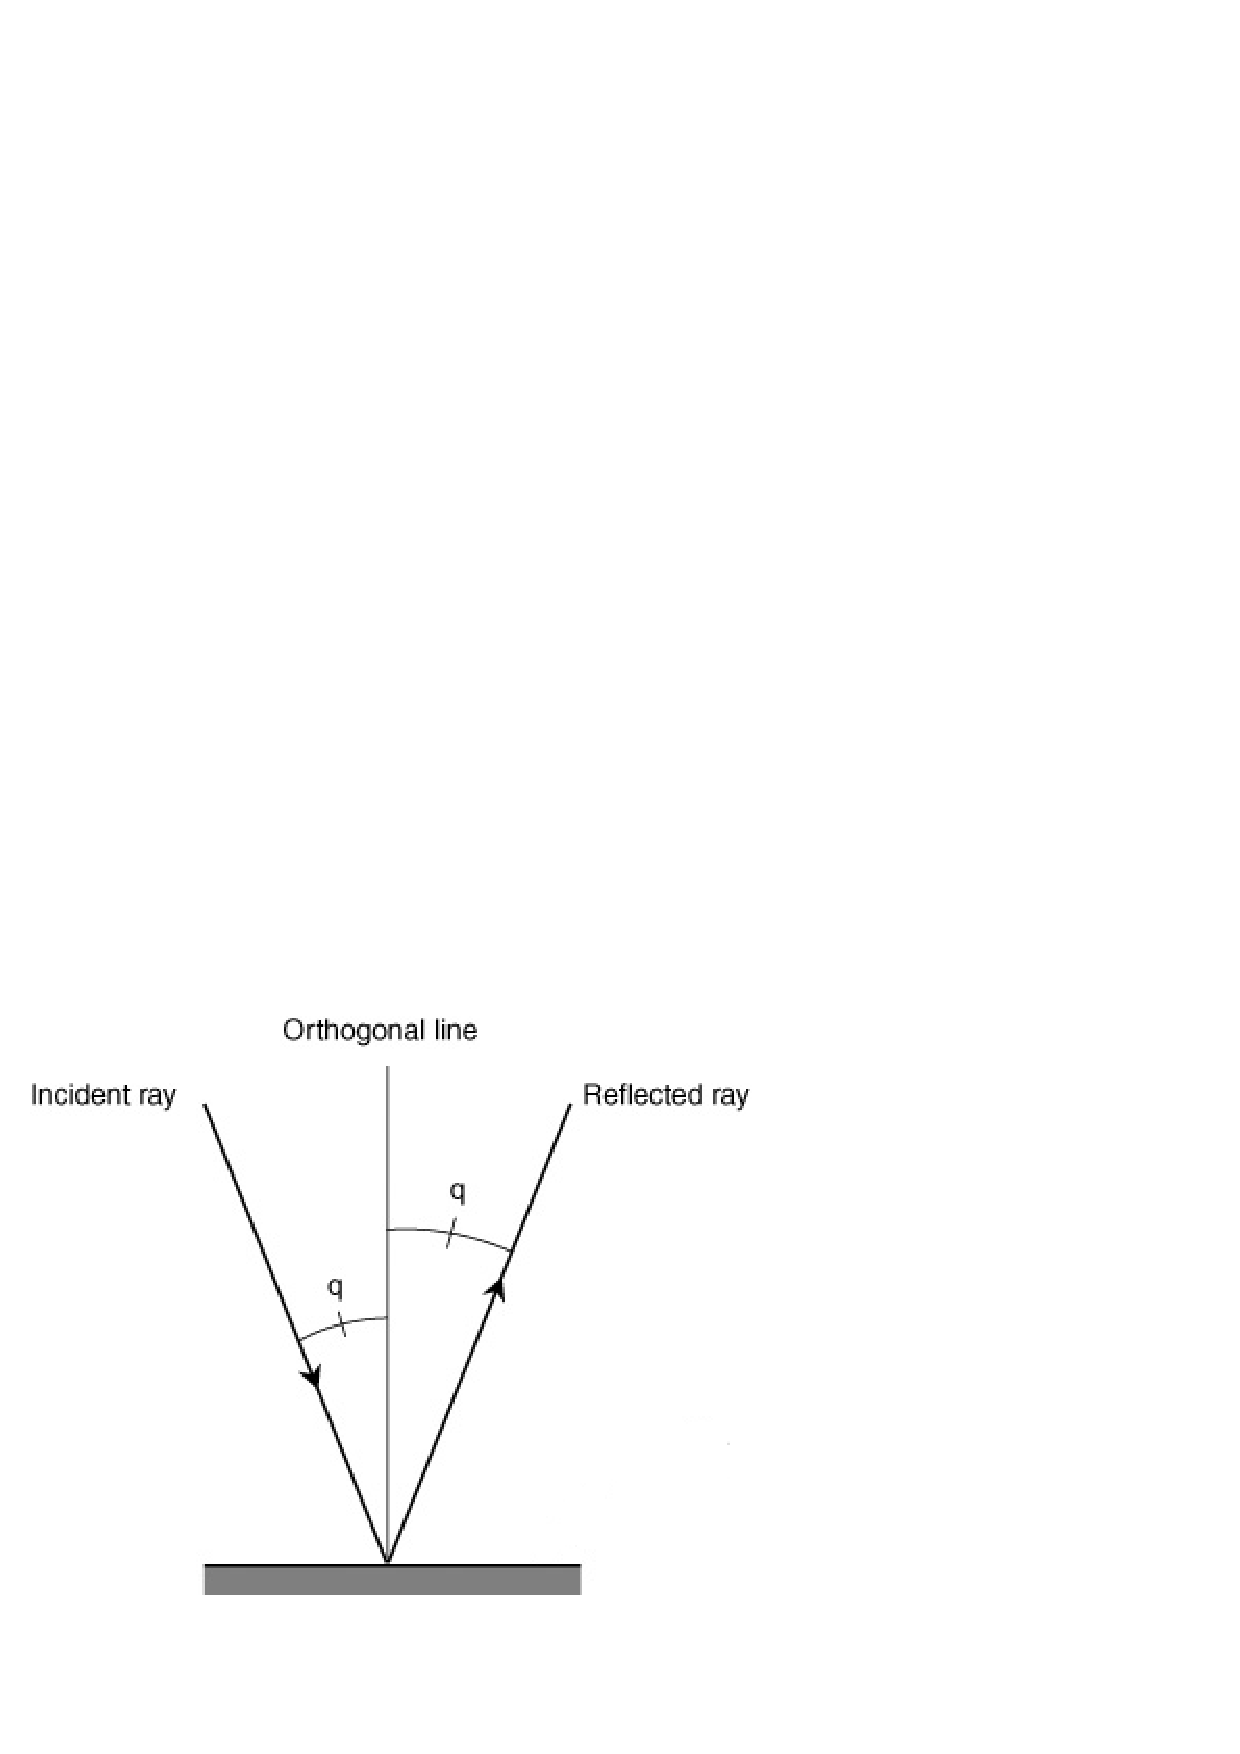
\includegraphics[keepaspectratio,width=2in]{particle_collision.png}
  \end{center}
  \vspace{-.2in} % corrects bad spacing
  \caption{\label{fig:collision-angle}Mechanics of the ball colliding with a table edge.}
\end{figure}

Introducing some notation to the problem, we will label the horizontal edges of the table $h$ and the vertical edges of the table $v$. Whenever the ball collides with a horizontal edge, we will call the resulting collision an $h$ collision. Likewise, collisions with vertical edges will be denoted as $v$ collisions.

\begin{definition}
  A \emph{collision sequence} ($\alpha$) for a ball is the sequence of sides that the ball collides with ($\alpha_i \in \cbracket{v, h}$). This sequence is ordered by increasing collision time. In this paper, ball trajectories are idealized and infinite, but we will only look at finite subsequences of the infinite collision sequences formed by these trajectories. Furthermore, we will only look at finite collision sequences that start and end with h.
\end{definition}

\subsection{An Example Collision Sequence}

For the reader to better understand the basic properties of collision sequences, we will consider an example trajectory and form a collision sequence from a short segment of the trajectory. Consider a ball with initial position $\bvec{x}_0 = (0.75, 0.75)$ and initial velocity $\bvec{u}_0 = (4.6, 1)$.

\begin{figure}[H]
  \begin{center}
    \includegraphics[keepaspectratio,width=3in]{example.png}
  \end{center}
  \vspace{-.2in} % corrects bad spacing
  \caption{\label{fig:example}Example trajectory, $x_0 = (0.75, 0.75)$, $u_0 = (4.6, 1)$.}
\end{figure}

The collision sequence corresponding to this trajectory segment is the following:

\begin{equation}
	\alpha = (v, h, v, v, v, v, v, h, v, v, v, v, v, h, v, v, v)
\end{equation}
